\documentclass[12pt,a4paper,parskip,listof=totoc,bibliography=totoc]{scrreprt}
\usepackage[english,german,ngerman]{babel}
\usepackage[utf8]{inputenc}
\usepackage[T1]{fontenc}
\usepackage{amsmath}
\usepackage{amsfonts}
\usepackage{amssymb}
%http://www.namsu.de/Extra/pakete/Setspace.html
\usepackage{setspace}
%Fußnoten werden das ganze Dokument über durchgezählt
%Quelle: http://golatex.de/nummerierung-der-fussnoten-durchgehend-im-gesamten-dokument-t2042.html
\usepackage{chngcntr}
\counterwithout{footnote}{chapter}
\usepackage{makeidx}
\makeindex
\usepackage{graphicx}
%Für Quellcodeschnippsel
%Für Bash Code Highlighting
\usepackage{minted}
%Anleitung: https://en.wikibooks.org/wiki/LaTeX/Source_Code_Listings
\usepackage{listings}
\usepackage{color}

\definecolor{mygreen}{rgb}{0,0.6,0}
\definecolor{mygray}{rgb}{0.5,0.5,0.5}
\definecolor{mymauve}{rgb}{0.58,0,0.82}

\lstset{ %
  backgroundcolor=\color{white},   % choose the background color; you must add \usepackage{color} or \usepackage{xcolor}
  basicstyle=\footnotesize,        % the size of the fonts that are used for the code
  breakatwhitespace=false,         % sets if automatic breaks should only happen at whitespace
  breaklines=true,                 % sets automatic line breaking
  captionpos=b,                    % sets the caption-position to bottom
  commentstyle=\color{mygreen},    % comment style
  deletekeywords={...},            % if you want to delete keywords from the given language
  escapeinside={\%*}{*)},          % if you want to add LaTeX within your code
  extendedchars=true,              % lets you use non-ASCII characters; for 8-bits encodings only, does not work with UTF-8
  frame=single,	                   % adds a frame around the code
  keepspaces=true,                 % keeps spaces in text, useful for keeping indentation of code (possibly needs columns=flexible)
  keywordstyle=\color{blue},       % keyword style
  language=Octave,                 % the language of the code
  otherkeywords={*,...},           % if you want to add more keywords to the set
  numbers=left,                    % where to put the line-numbers; possible values are (none, left, right)
  numbersep=5pt,                   % how far the line-numbers are from the code
  numberstyle=\tiny\color{mygray}, % the style that is used for the line-numbers
  rulecolor=\color{black},         % if not set, the frame-color may be changed on line-breaks within not-black text (e.g. comments (green here))
  showspaces=false,                % show spaces everywhere adding particular underscores; it overrides 'showstringspaces'
  showstringspaces=false,          % underline spaces within strings only
  showtabs=false,                  % show tabs within strings adding particular underscores
  stepnumber=1,                    % the step between two line-numbers. If it's 1, each line will be numbered
  stringstyle=\color{mymauve},     % string literal style
  tabsize=2,	                   % sets default tabsize to 2 spaces
  title=\lstname                   % show the filename of files included with \lstinputlisting; also try caption instead of title
}
%head statt top bringt exakt 4cm Abstand am Kopf
\usepackage[left=4.00cm, right=2.00cm, head=4.00cm, bottom=2.00cm]{geometry}
%Glossar anschalten und in TOC aufnehmen und erzeugen
%https://en.wikibooks.org/wiki/LaTeX/Glossary
\usepackage{hyperref} %Klickbare Einträge im Glossar
%\usepackage[toc,acronym]{glossaries}
%\makeglossaries
%\usepackage[nomain,acronym,xindy,toc]{glossaries} % nomain, if you define glossaries in a file, and you use \include{INP-00-glossary}
%http://tex.stackexchange.com/questions/111192/problems-with-xindy-and-glossaries
%\usepackage[nonumberlist,nomain,acronym,toc]{glossaries}
% Acronym muss an erster Stelle stehen, sonst funktioniert die Trennung von Abkürzungsverzeichnis und Glossar nicht
\usepackage[acronym,nonumberlist,toc]{glossaries}
%Glossareinträge
\newglossaryentry{GPLv2}
	{
 	 name=GPLv2,
 	 description={is a programmable machine that receives input,
               stores and manipulates data, and provides
               output in a useful format}
	}
\newglossaryentry{psu}
	{
	name=PSU,
	description={Power Supply Unit, Netzteil},
	plural=PSUs
	}
\newglossaryentry{sla}
	{
	name=SLA,
	description={Service Level Agreement}
	}
%Glossareinträge Ende
%Acronyme
\newacronym{rz}{RZ}{Rechenzentrum}
\newacronym{ram}{RAM}{Random Access Memory}
\newacronym{ca}{CA}{Computer Associates}
\newacronym{fc}{FC}{Fibre Channel}
\newacronym{elk}{ELK}{Elasticsearch - Logstash - Kibana}
\newacronym{it}{IT}{Informationstechnik}
\newacronym{omd}{OMD}{Open Monitoring Distribution}
\newacronym{os}{OS}{Betriebssystem}
\newacronym{etc}{etc.}{etcetera}
\newacronym{itil}{ITIL}{Information Technology Infrastructure Library}
\newacronym{sla}{SLA}{Service Level Agreement}
\newacronym{snmp}{SNMP}{Simple Network Management Protocol}
\newacronym{dv}{DV}{Datenverarbeitung}
\newacronym{bspw}{bspw.}{beispielsweise}
\newacronym{zb}{z.B.}{zum Beispiel}
\newacronym{nrpe}{NRPE}{Nagios Remote Plugin Executor}
\newacronym{san}{SAN}{Storage Area Network}
\newacronym{psu}{PSU}{Power Supply Unit}
\newacronym{rest}{REST}{Representational State Transfer}
\newacronym{api}{API}{Application Programming Interface}
\newacronym{cpu}{CPU}{Central Processing Unit}
\newacronym{itsm}{ITSM}{IT Service Management}
\newacronym{llc}{LLC}{Limited Liability Company}
\newacronym{obs}{OBS}{Open Build Service}
\makeglossaries
%\usepackage{imakeidx}
%Tiefe der Nummerierung ändern, Subsubsection ist Ebene 3
\setcounter{secnumdepth}{4}
\setcounter{tocdepth}{4}
% Bibliothek & Zitierstil
\usepackage[style=authortitle-icomp,backend=biber]{biblatex}
\usepackage[babel,german=guillemets]{csquotes}
%\bibliography{seminararbeit_monitoring.bib} %U.u. deprecated
% Anleitung zu BibLaTEX: http://biblatex.dominik-wassenhoven.de/download/DTK-2_2008-biblatex-Teil1.pdf
\addbibresource{seminararbeit_monitoring.bib}
%So werden URLs im Literaturverzeichnis in eine neue Zeile geschrieben
%Quelle: http://www.golatex.de/biblatex-literaturverzeichnis-zeilenumbruch-vor-url-t8406.html
\DeclareFieldFormat{url}{\newline URL: \url{#1} }
\setuptoc{toc}{bibliography=totoc}
% Abkürzungsverzeichnis mit Nomencl
% siehe http://texwelt.de/wissen/fragen/4942/wie-kann-ich-die-erstellung-eines-abkurzungsverzeichnisses-mit-dem-paket-nomencl-automatisieren
% und http://golatex.de/abkuerzungsverzeichnis-mit-texmaker-t8301.html
% Zum aktualisieren muss "Makeindex" aufgerufen werden, Konfiguration siehe letzter Link
%\usepackage[intoc]{nomencl}
% Befehl umbenennen in abk
%\let\abk\nomenclature
% Überschrift
%\renewcommand{\nomname}{Abkürzungsverzeichnis}
% Punkte zw. Abkürzung und Erklärung
%\setlength{\nomlabelwidth}{.20\hsize}
%\renewcommand{\nomlabel}[1]{#1 \dotfill}
% Zeilenabstände verkleinern
%\setlength{\nomitemsep}{-\parsep}
%\makenomenclature
% Ende Abkürzungsverzeichnis

%\usepackage{showframe}% zum Anzeigen des Seitenlayouts

%% Abstände um Chapter
%\RedeclareSectionCommand[beforeskip=-1\baselineskip,afterskip=.5\baselineskip]{chapter}

%\pagestyle{headings}
%Schriftgrößen noch ein wenig anpassen...
\setkomafont{chapter}{\fontsize{16bp}{18.8bp}\selectfont}
\setkomafont{section}{\fontsize{14bp}{18.8bp}\selectfont}
%\addtokomafont{disposition}{\hspace*{1.5cm}}
\renewcommand{\chapterheadstartvskip}{\vspace*{-1\topskip}}
\renewcommand{\chapterheadendvskip}{\vspace*{0.2\topskip}}
\renewcommand*{\chapterheadstartvskip}{\vspace*{-\topskip}}

\begin{document}
	%TODO: Titelseite an die Erfordernisse anpassen
	%http://golatex.de/wiki/Widmung
	\subject{Seminararbeit im Studiengang \glqq Verwaltungsinformatik\grqq}
	\author{Markus Österle}
	\title{Servermonitoring in Rechenzentren}
	\subtitle{am Beispiel von Linux Systemen}
	\publishers{Betreut von Dipl. Inf. Stefan Müller}
	\date{} % setzt ein leeres Datum und löscht quasi das per default verwendete \today von der Titelseite

	\maketitle
	
	\tableofcontents
	% Gibt das Latex Logo aus...Stelle? 
	%\LaTeXe{}
	%Ab hier 1.5facher Zeilenabstand 
	\onehalfspacing
	\chapter{Einleitung}
	Das Thema des Servermonitorings hat sich im professionellen \acrshort{it} Umfeld in den letzten Jahren zu einem großen Thema entwickelt. Durch die steigende Abhängigkeit nahezu aller Bereiche unseres Lebens von \acrshort{it}-Systemen steigen auch die Anforderungen an die Verfügbarkeit und die Performance und somit auch an die Überwachung der selbigen. Reichte es in den 90er Jahren noch aus von einem zentralen Rechner (gemeint ist hier ein normaler Personal Computer) per Ping zu überwachen ob die Server verfügbar sind, so wird heute ein sehr viel feineres Monitoring erwartet. Nicht nur die Erreichbarkeit der Rechner soll überwacht und statistisch aufbereitet werden, sondern auch die Auslastung und die Gesundheit einzelner Bauteile (bspw. \acrlong{psu}s (Netzteile), \acrshort{ram} Bausteine; \acrshort{cpu}, Festplatten), soll lückenlos überwacht werden. Um eine schnelle Reaktion auf eventuell auftretende Fehler zu ermöglichen. 

	In der vorliegenden Arbeit wird das Thema und die Historie des Servermonitorings in Rechenzentren betrachtet. Zur Begrenzung des Themengebiets wird dezidiert ausführlicher auf das Teilgebiet der Überwachung von *nix-Systemen eingegangen. Dies hat zum einen den Grund, dass der Autor viele Jahre Erfahrung mit Linux und Unix Betriebssystemen vorweisen kann und schon einige Erfahrung mit der Überwachung von *nix-Servern gemacht hat und zum anderen ermöglicht diese Eingrenzung eine tiefergehende Beschäftigung mit wenigstens einem Themengebiet.
	\section{Warum Monitoring im Rechenzentrum?}
	%TODO kritische Betriebszustände definieren?
	Aus der Sicht eines Systemadministrators (in Folge nur noch Admin genannt) macht es eigentlich von Grunde auf Sinn so viele Informationen wie nur möglich über seine Systeme zu haben:
	\begin{itemize}
		\item Wie sind meine Server ausgelastet?
		\item Ist die Hardware in Ordnung?
		\item War der gestrige Ansturm auf die Homepage zu verkraften?
		\item Zeigen meine Server ungewöhnliches Verhalten?
		\item Ist meine Sicherheitssoftware up to date?
	\end{itemize}
	  All diese Fragen könnten über ein richtig eingesetztes und konfiguriertes Monitoringsystem schnell und sicher beantwortet werden. Darüber hinaus ermöglicht ein solches System dem Admin schnell auf kritische Betriebszustände (\acrlong{bspw} Netzteil im Server oder Festplatte im RAID ausgefallen) zu reagieren und diese zu beheben, was sich positiv bei der Ausfallzeit seiner Systeme bemerkbar macht. 
	  
	  Ein ebenfalls positiver Nebeneffekt ist, dass ein gutes Monitoring den Admin in die Lage versetzt schnell (grafisch) aufbereitetes Material zur Verfügung stellen zu können, mit dem man zum Beispiel nachweisen kann, dass die Systeme dringend aufgerüstet werden müssen oder das Performanceprobleme manchmal eben doch an schlecht programmierter Software und nicht an den Systemen liegt.
	  
	\section{Warum Linux?}
	Systemüberwachung ist natürlich für alle Komponenten im Rechenzentrum wichtig, begonnen bei der Basisversorgung (Strom, Kühlung) über die grundlegende Infrastruktur (Netzwerkinfrastruktur, evtl. Storageinfrastruktur) bis zu den einzelnen Systemen (natürlich quer über die Betriebssystemgrenzen hinweg). Mit den später in dieser Arbeit vorgestellten Lösungen könnten viele dieser Felder abgedeckt werden, eine genaue Beschreibung des wie würde allerdings den (sowohl den zeitlichen als auch den mengenmäßigen) Rahmen der Arbeit sprengen, wie bereits in der Einleitung erwähnt. 
	
	Deshalb werden wir uns nach den allgemeinen Definitionen und Einführungen in den Themenkomplex \glqq Monitoring\grqq\ auf das Thema der Serverüberwachung von Linux Systemen spezialisieren. Dies ist ein relativ dankbares Gebiet für diese Ausführungen da man relativ gut die Mächtigkeit und Schlagkraft eines richtig konfigurierten Monitoringsystems zeigen kann. Für Linux spricht auch, dass es zum einen eine relativ große Verbreitung im Serverbereich hat und die Arbeit auch für den privaten Gebrauch nicht irrelevant ist, da der Überwachung mit den vorgestellten Tools keine Grenzen gesetzt sind durch den modularen Aufbau und die Erweiterbarkeit mit selbstgeschriebenen Skripten, Plugins, \acrshort{etc}. sind der Phantasie keine Grenzen gesetzt. Die Systeme können beispielsweise ohne großen Aufwand und geistige Eigenleistung (Anleitungen und Code für vieles gibt es bereits im Netz) für die Überwachung privater Webservices, privater Netzwerkinfrastrukturen, SmartHomes, Wetterstationen, \acrshort{etc} genutzt werden.
	%TODO Verbreitung von Linux im Serverbereich Grafik und Quelle,wohl knapp unter 50% im Serverbereich
		
	
	\chapter{Vom Ping zum proaktiven Monitoring}
	In den folgenden Unterkapiteln werde ich mich mit der grundlegenden Definition von Begriffen rund um das Thema Monitoring/Serverüberwachung beschäftigen und einen kleinen Überblick über die Historie geben.
	\section{Historie}
	%TODO Ausformulieren und deutsche Sätze draus machen
	Zu Beginn der IT Zeit, als Server noch Mainframes und sehr teuer waren und wenige spezialisierte Anwendungen auf ihnen betrieben wurden, war die Überwachung dieser Systeme für die Administratoren ein kleiner Aufwand. Die Administratoren waren über ihre Terminals meistens sowieso direkt mit dem Mainframe verbunden und sahen (in der bedienten Betriebszeit) etwaige Fehlermeldungen sofort auf ihren Konsolen. Dies hat sich im Wandel der Zeit drastisch verändert, die großen Mainframes von einst werden durch eine Vielzahl von kleineren Servern ersetzt um die gestiegenen Anforderungen erfüllen zu können. Wo früher auf einem Rechner (mit der entsprechenden Hot-/Cold-Standby-Lösung wenn die Firma/Behörde) die Datenbanken für die komplette Firma liefen, werden diese heute durch eine Vielzahl an Datenbanksystemen (die unter Umständen auch noch Hochverfügbar ausgelegt sind) ersetzt. Dies und die Tatsache, dass ohne diese IT Systeme in vielen Bereichen nicht mehr funktioniert führt natürlich auch zu ganz anderen Anforderungen an Verfügbarkeit und damit auch an die Erkennung von Fehlern und Ausfällen. 
	
	Während es früher ausreichend war, mit einer selbst gestrickten (Skript-)Lösung per \textit{Ping} zu überwachen ob alle Server erreichbar sind und bei einem Fehler der Admin sich selbst in den Serverraum gehen musste um den Rechner und seine Fehlermeldung in Augenschein zu nehmen muss es heute etwas detaillierter sein. Zumindest die Anwendungen die für den Betrieb kritisch sind müssen überwacht werden um Fehler und Ausfälle schnell erkennen und beheben zu können, unter Umständen möchte man auch einfach bei Ausfall einer Anwendung eine automatische Aktion auslösen (z.B. einen automatischen Neustart des Webservers). Auch die Fehlermeldung soll nach Möglichkeit bereits im Monitoring erkennbar sein.
	
	Das (lokale) Monitoring von Performanceparametern war in der Geschichte der *nix Betriebssysteme schon immer möglich, der Komfort und die Zahl der Tools hat sich über die Jahre gesteigert. Tools wie \textit{top} haben ihren Ursprung in den 80er Jahren\footcite{top} (lauffähig unter Unix), also sogar vor der Entwicklung von Linux (ab 1991). Das Sysstat Paket mit Tools wie \textit{iostat} für das Monitoring der Festplattenaktivität und \textit{SAR} für fortlaufendes Schreiben von Performance Daten per Cronjob gibt es seit 06.03.1999\footcite{sysstatchangelog}.
	%TODO Wo wollen wir hier hin?
	Cacti und RRDTool
	Systemlogs die in ihrer Vielzahl unüberblickbar sind und um Sie überhaupt verarbeiten zu können auf jeden Fall gefiltert und aufbereitet werden müssen. Verschiedene Logserver (Syslog-ng, rsyslog, systemd).
	
	Auch eine zunehmende Standardisierung der IT Prozesse wie beispielsweise \acrfull{itil} und die damit verbundenen Pflichten zur Messung bestimmter Größen tragen ihren Teil zur Notwendigkeit von immer umfangreicheren Monitoring- und Reportingsystemen bei. Auf \acrshort{itil} gehen wir im folgenden Kapitel noch einmal ausführlicher ein.
	%\subsection{ITIL die Quelle allen Übels?}
	%Definition ITIL - ITIL \& Monitoring?
	%\acrfull{itil}
	
	\section{Definitionen rund um das Thema (Server-/System-)Monitoring}
	Was verbirgt sich nun hinter magischen Begriffen wie \acrshort{itil} und Monitoring, in der Folge werde ich versuchen die gebräuchlichsten Definitionen darzulegen und zu beschreiben wie die einzelnen Spielarten des Monitorings mittels Tools im praktischen Teil der Arbeit umgesetzt werden.
	\subsection{ITIL}
	Die Begrifflichkeit \acrshort{itil} wird uns in der Folge noch öfter über den Weg laufen. Ausgeschrieben heißt \acrshort{itil}: \acrlong{itil} und ist eine über Jahrzehnte gewachsene Sammlung von Best Practices zum Thema IT Service Management\footcite{ebelitilv3}. \glqq\acrfull{itsm} nutzt Methoden, die nötig sind, um die bestmögliche Unterstützung von Geschäftsprozessen durch die IT-Organisation zu erreichen. \acrshort{itil} ist der diesbezüglich genannte De-facto-Standard\grqq\footcite[S. 27]{ebelitilv3}, was aber nicht gleichzusetzen ist mit einem offiziellen Standard. 
	Services was ist das? Unter Service versteht man bei \acrshort{itil} die Gesamtheit der physischen und logischen (IT- und nicht IT-) Komponenten, die benötigt werden, um die Unterstützung ausgewählter Geschäftsprozesse sicherzustellen.\footcite{sommeritservicemgmt}
	Alles dreht sich darum Qualität des IT Services zu verbessern.
	
	%https://de.wikipedia.org/wiki/ITIL_V3_Service_Operation
	ITIL Service Operation? 
	
	Für eine vernünftige Einführung von \acrshort{itil} im Unternehmen ist ein funktionierendes Monitoring- und Reportingsystem unbedingt notwendig.
	\subsection{Monitoring - Allgemein}
	%TODO Definition Monitoring
	Laut dem Duden handelt sich beim Monitoring um
	\begin{center}
		\glqq[Dauer]beobachtung (eines bestehenden Systems)\grqq\footcite[S. 701; Stichwort Monitoring]{duden}
	\end{center}
	Dieser Definition ist auch aus Informatikersicht nicht mehr allzu viel hinzuzufügen, außer dass es sich natürlich in unserem Fall um die Beobachtung eines \acrshort{it}-Systems handelt. Unter diese Definition fällt sowohl die temporäre Beobachtung, wie sie \acrlong{bspw} mit \textit{top} realisiert werden kann als auch eine dauerhafte Beobachtung bei der gesammelte (Performance-)Daten von einzelnen Rechner per Skript, Agent oder ähnlichem an ein zentrales System übertragen werden, wo sie gespeichert und ausgewertet werden.
	
	\subsection{reaktives Monitoring}
	\glqq Reaktives Monitoring ist eine Form der Überwachung, bei der als Reaktion auf ein bestimmtes Event entsprechende Maßnahmen eingeleitet werden. Beispielsweise die Auslösung eines Batchjobs, sobald ein vorheriger Batchjob abgeschlossen wurde, oder die Erfassung eines Incidents, wenn ein Fehler auftritt\grqq
	\footcite[S. 511]{ebelitilv3}
	
	Die Begrifflichkeit des Incidents kommt aus der \acrshort{itil}-Welt und bezeichnet die Eröffnung eines Fehlertickets in einem Ticketsystem und die Weiterleitung des selbigen an die zuständige Stelle, wenn eine Störung auftritt. Die Auslösung eines Batchjobs ist in Nagios zwar möglich, aber normalerweise wird man für die Zwecke der Arbeits-/Auftragsverwaltung (auch Job Steuerung genannt) speziellere Systeme verwenden. Was allerdings möglich ist, ist \acrlong{bspw} bei Systemen bei denen kein Datenverlust (zumindest wenn man abgebrochene Sitzungen der Benutzer außen vor lässt) droht einen automatischen Neustart durchzuführen sobald diese Abstürzen oder ungewöhnliches Verhalten zeigen, mit einer solchen Vorgehensweise könnten u.U. Benachrichtigungen von teuren Rufbereitschaftskräften abgesehen werden.
	 
	\subsection{proaktives Monitoring}
	%http://www.thefreedictionary.com/proactive
	\glqq Proaktives Monitoring ist eine Form der Überwachung, bei der versucht wird, Event-Muster zu ermitteln, um mögliche zukünftige Ausfälle zu prognostizieren.\grqq \footcite[S. 511]{ebelitilv3}
	
	Nach meiner Auffassung stellt ein richtiges proaktives Monitoring die Königsdisziplin innerhalb des Monitorings dar. Zwar hat sich die (Überwachungs-)Software und die Vielzahl der verfügbaren Agenten (siehe spätere Kapitel) in den letzten Jahren stark verbessert und die dadurch gestiegene Vielzahl an verfügbaren Informationen erleichtert einiges. Aber es Bedarf immer noch einer kundigen Hand, die die jeweiligen Filter definiert, damit das System beim überschreiten kritischer Werte Alarm schlägt. \footcite{Borkmann2009}
	
	Um ein vernünftiges proaktives Monitoring realisieren zu können brauche ich für die Analyse immer die größtmögliche Anzahl an Informationen, eine breitere Datenbasis erleichtert die Einschätzung des Fehlers. Deshalb halte ich es in diesem Fall für richtig und wichtig, nicht nur Performancedaten und Daten über den Status der einzelnen Anwendungen zu sammeln und auszuwerten, sondern auch die System- und Anwendungslogs nach kritischen Mustern zu durchsuchen und ggf. Alarm zu schlagen.
	%TODO Mustererkennung vor Ausfall, Borkmann einbauen
	\subsection{Verfügbarkeitsmonitoring}
	Verfügbarkeitsmonitoring bezeichnet die Überwachung der Verfügbarkeit, einer Anwendung oder eines Servers, d.h. die Beantwortung der Frage \glqq Wie lange war der Server/die Anwendung für den Kunden erreichbar\grqq\. Das Monitoring der Verfügbarkeit kann ein Teil des SLA-Monitorings sein, wenn im SLA eine spezifische Verfügbarkeit vereinbart wurde, darauf gehen wir im nächsten Abschnitt noch näher ein, wenn wir uns mit dem Thema SLA-Monitoring noch näher beschäftigen.
	\subsection{SLA Monitoring}
	Unter einem \acrfull{sla} versteht man in ITIL eine \glqq Vereinbarung zwischen einem \acrshort{it} Service Provider und einem Kunden, der einen zu erbringenden Service und dessen Service Level inklusive Service Level-Zielen, Verantwortlichkeiten von \acrshort{it} Service Provider und Kunde genau definiert. Ein \acrshort{sla} kann mehrere IT Services oder Kunden abdecken.\grqq \footcite[S. 732; Stichwort: Service Level Agreement]{ebelitilv3} Die im \acrshort{sla} vereinbarten Service Level-Ziele sollten SMART sein und auf KPIs basieren, d.h. mess- und überprüfbar sein.\footcite[S. 733; Stichwort: Service Level-Ziele]{ebelitilv3}
	
	Beim SLA Monitoring geht es darum die Einhaltung der vereinbarten Service Level-Ziele zu überwachen und sinnvoller Weise in Form von Reportings für die Kunden und die Kollegen vom Service Level Management (die Stelle die lt. \acrshort{itil} für die Verhandlung und Vereinbarung des \acrshort{sla} zuständig ist) aufzubereiten und zur Verfügung zu stellen.
	%TODO Fußnote noch an den Text nach oben ziehen.
	Einhaltung vereinbarter Servicelevel \footcite[40]{iso20000sla}
	\subsection{Fazit}
	%TODO ITIL Begrifflichkeit vs. technische Begrifflichkeit, also proaktiv, reaktiv, SLA vs. Basis, erweitertes, spezialisiertes Monitoring
	Um alle in den vergangenen Unterkapiteln beschriebenen Anforderungen zu erfüllen ist es notwendig mehrere Überwachungstechnologien zu verbinden, um ein optimales Monitoring zu erhalten. So ist es zur proaktiven Erkennung von Fehlern zum einen unerlässlich die Einträge in Logfiles auswerten zu können, um Fehler zu bemerken lange bevor Sie beginnen sich auf den Produktivbetrieb auszuwirken (bspw. Schreibfehler auf ein per \acrlong{fc} (\acrshort{fc}) angebundenes \acrshort{san}-System oder einfach I/O Fehler auf eine der Systemfestplatten) und zum anderen auch die Performance der Systeme im Auge zu behalten um sicher zu stellen, dass die Dimensionierung der Systeme richtig ist und nicht plötzliche Engpässe auftreten können. Dies ist vor allem durch die grafische Aufbereitung und historische Speicherung der Daten möglich. 
	\chapter{Monitoring Systeme für Linux Server}

	Nachdem wir im vorherigen Kapitel einige grundlegende Begriffe bereits geklärt haben, ist es nun an der Zeit uns Gedanken darüber zu machen, wie ein Monitoring aussehen könnte und was es alles leisten sollte. 
	\section{Grundlegende Überlegungen}
	Die wesentlichen Fragen\footcite[nach][]{veltnagios1} vor Beginn einer Implementierung einer Monitoring Lösung sollten sein:
	\begin{itemize}
		\item Was soll überwacht werden?
		\item Wie kann überwacht werden?
		\item Wer soll im Fehlerfall benachrichtigt werden?
		\item Welche Service Level Agreements existieren bereits, welche sollen in naher Zukunft abgeschlossen werden?
		\item Welche Software ist für meine Zwecke am besten geeignet?
	\end{itemize}
	\subsection{Was soll überwacht werden?}
	Hier kann man die Themenbereiche grob in drei Stufen der Überwachung einteilen, die drei Stufen gruppieren die Anforderungen entsprechend dem Aufwand
	\begin{itemize}
		\item Grundlegende Überwachung
		
		Stufe mit dem wenigsten Aufwand, hier wird im wesentlichen kontrolliert ob alle Server und Serverdienste erreichbar sind und ob die Netzwerkinfrastruktur in Ordnung ist.\\
		\textbf{Mit TCP/IP realisierbar}
		\item Erweiterte Überwachung
		
		Beispielsweise Auslastung von Routern \& Switchports oder Auslastung von Servern, freier Platz auf Festplatten, Datenbanken\\
		\textbf{Mit Hilfe von speziellen Protokollen, z.B. \acrshort{snmp} oder applikationsbezogenen Werkzeugen realisierbar}
		\item Spezialisierte Überwachung
		
		Temperaturüberwachung der \acrshort{dv}-Räume, Qualität der Stromversorgung, aktuelle Netzlast der einzelnen Serverräume\\
		\textbf{Nur mit individueller Hard- und Software realisierbar (Beispielsweise Überwachungsmodule in den Schaltschränken und Sensorik in den Rechnerräumen )}
	\end{itemize}
	\subsection{Wie kann überwacht werden?}
	Im wesentlichen können an dieser Stelle zwei Arten der Überwachung unterschieden werden:
	\begin{itemize}
		\item Aktive Überwachung
		\begin{itemize}
		\item In regelmäßigen Abständen werden Programme ausgeführt, die eine Überprüfung durchführen
		\item Die Rückgabewerte werden ausgewertet
		\item Besteht ein Fehler über längere Zeit (bzw. über einen definierten Zeitraum hinaus) wird ein Zuständiger informiert
		\end{itemize}
		\item Passive Überwachung
		\begin{itemize}
			\item Ein Dienst, Server, Agent, o.ä. meldet einen Fehler
			\item Die Eingabe wird ausgewertet
			\item Je nach Ereignis und Konfiguration wird ein Zuständiger informiert
		\end{itemize}
	\end{itemize}
	\subsection{Wer soll im Fehlerfall benachrichtigt werden?}
	Diese Frage ist in den meisten (größeren) Unternehmen und Behörden gar nicht so einfach zu beantworten, da die Aufgabengebiete unterteilt sind und es unter Umständen schwierig ist die passende Person zu informieren, da die (technische) Abbildung von Zuständigkeiten an vielen Stellen kompliziert bis nicht möglich ist. 
	
	Weiter stellt sich das Problem das nicht bei jedem Ausfall die gleichen Personen zu benachrichtigen sind:
	So kann es sich beim Ausfall eines Servers um vielfältige Probleme handeln, \acrlong{bspw} ein Betriebssystem- oder ein Netzwerkproblem.
	Außerdem muss festgelegt werden ob und wer 24/7 (also 24h am Tag, sieben Tage die Woche) über aufgetretene Fehler informiert werden muss/soll.
	\subsection{Welche Service Level Agreements existieren bereits, welche sollen in naher Zukunft abgeschlossen werden?}
	Diese Information ist besonders wichtig um festlegen zu können welche Kennzahlen ich auf jedem Fall aus meinem Monitoring bekommen will um den Anforderungen gerecht zu werden.
	\subsection{Welche Software ist für meine Zwecke am besten geeignet?}
	Bei der Recherche nach Monitoringtools für Linux Systeme stößt man auf verschiedenste Lösungen, da wären zum einen die Lösungen die lokal auf jedem Server zu installieren sind, der Performance Monitor \textit{top} und seine Derivate (atop, iotop, htop, ntop) oder das Systat-Paket\footcite{sysstat} mit seinen Komponenten (\acrlong{bspw} SAR\footcite{sarkrenn}, iostat). Allerdings haben alle diese Programme das Problem, dass ich mich auf dem Server anmelden muss um Informationen zu bekommen, einzig bei SAR hätte ich die Möglichkeit, die per Cronjob generierten Dateien per Skript einzusammeln und auf einem zentralen Server mit einem Tool wie KSar\footcite{ksar} grafisch auszuwerten oder KSar die Daten selbst einsammeln zu lassen indem ich mich auf dem Server anmelde wenn ich Performance Daten brauche. Dies ist allerdings nicht wirklich befriedigend da es bei diesen Lösungen um ein reines Monitoring von Performancedaten geht und nicht um ein Monitoring der Verfügbarkeit bestimmter Dienste oder die Benachrichtigung/Alarmierung im Fehlerfall. Um eine solche Funktionalität zu erhalten brauchen wir ein zentrales System. 
	%TODO Quelle für die per Cronjob generierten Dateien?
	Wenn man zu dem Thema \glqq zentrales Monitoringsystem für Linux\grqq\ im Internet recherchiert wird man neben den diversen teuren Softwarelösungen diverser Hersteller (z.B. \acrlong{ca} Unified Monitoring oder Microsoft SCOM) immer wieder über einen Namen stolpern: Nagios. Das Tool hat sich fürs Monitoring von Linux Systemen zu einer Art Industrie Standard entwickelt. Das mag zum einen an seiner freien Verfügbarkeit liegen, zum anderen aber vielleicht auch daran, dass im Linux Umfeld viele Administratoren die Quelloffenheit und die leichte Erweiterbarkeit mittels eigener Tools, Plugins, Agenten von Nagios schätzen. Darüber hinaus findet man ein weites Angebot an Support und Serviceleistungen, sowohl im Internet, als auch von Consultingfirmen, die meist auch an der Entwicklung der Systeme beteiligt sind. Und wahrscheinlich der gewichtigste Vorteil gegenüber allen Mitbewerbern, eine Nagios Installation kostet erstmal nichts, ic hbrauche lediglich einen Server auf dem ich die Software installieren kann und einen Administrator der gewillt ist sich in die Konfiguration einzuarbeiten. 
	
	Die eigentlich schon sehr gut und ausgereifte Architektur von Nagios auf der einen Seite und die immer wieder auftretenden Querelen bei der Entwicklung von Nagios, haben zu einer Vielzahl an Forks (als Fork bezeichnet man in der Softwareentwicklung eine Aufspaltung eines Projekts in zwei unterschiedliche voneinander unabhängige Projekte, die voneinander unabhängig weiterentwickelt werden) geführt. 
	Einige dieser Forks sind:
	\begin{itemize}
		\item \textbf{Icinga} 
		
		Entstanden 2009 aus Frust über die schleppende Weiterentwicklung von Nagios als Fork\footcite{icingaabspaltung}, Version 2 wurde von Grund auf neu entwickelt (\glqq from scratch\grqq), die Software soll aber so lange wie möglich kompatibel zu Nagios bleiben.\footcite{icingafaq}
		\item \textbf{Shinken}
		
		vollständige Portierung von Nagios in die Programmiersprache Python, Umstellung von Original Nagios auf Shinken sind ohne großen Aufwand möglich, da sowohl die Plugins, als auch die Konfigurationsdateien weiterhin funktionieren \footcite{shinkenabout}
		\item \textbf{Naemon}
	\end{itemize} gesorgt. Für die weitere Arbeit, gehen wir davon aus, dass die Auswahl in die Richtung Nagios gefallen ist, im nächsten Kapitel werden wir uns damit beschäftigen welche Möglichkeiten wir haben und welchen Funktionsumfang uns Nagios bietet.
	
	
	\section{Performance \& SLA Monitoring}
	%TODO: Warum Check_MK, warum nicht OMD, Vielfalt der Systeme OMD, Check_MK, OMD Lab Edition, bei ursprünglicher OMD auf der Seite nichts passiert, hinter den Kulissen aber schon, warum empfiehlt es sich trotzdem über eine Subskription nachzudenken (Förderung OS Gedanken, Professionieller Support und Schulung, mehr Features die erst später irgendwann in der freien Version ankommen)
	\subsection{Nagios}
	%TODO: Nagios als Kern, mit wenigen zusätzlichen Funktionen, die Funktionsumfänge die wir in der großen Version sehen werden mit externen Programmen realisiert.
	%TODO: Funktionsweise von Nagios kurz erläutern, aktive & passive Checks, auf Bild 3.1 Bezug nehmen, sollte für eine kurze Erläuterung absolut ausreichend sein.
	\begin{figure}[!h]
	\centering
	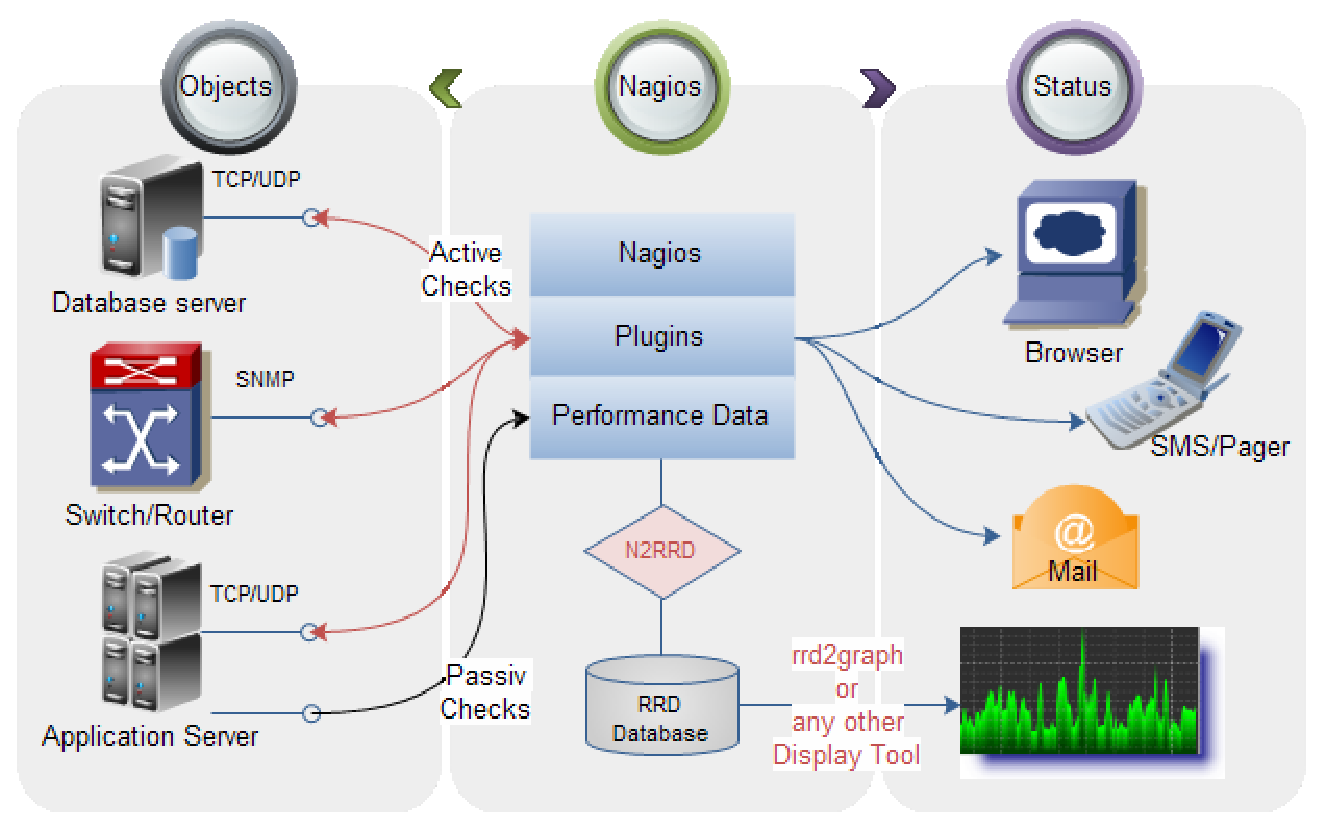
\includegraphics[width=1\textwidth]{pics/NagiosMonitoring.eps}
    \caption[Grober Aufbau von Nagios]{Aufbau einer Nagios Appliance (Quelle: \textcite{nagiosaufbau}}
    \label{fig:nagiosaufbau}
	\end{figure}
	\clearpage
	\subsubsection{Historie}
	Die Wurzeln von Nagios gehen zurück ins Jahr 1996 als Ethan Galstad ein MSDOS Programm schreibt, dass die Erreichbarkeit von Novell Netware Servern per \textit{ping} testet. Er verwendete hierbei schon das Konzept, dass er externe Tools (\textit{ping}) nutzt um die Überprüfungen (\glqq Checks\grqq) durchzuführen, dies ist bis heute das Basisarchitekturkonzept von Nagios.
	
	Die Programmierarbeiten am Vorgänger von Nagios begannen im Jahr 1998, als Galstad beschloß in das Geschäft mit Monitoringsystemen einzusteigen. Die verbesserte Applikation lief unter Linux und wurde im Jahr 1999 unter dem Namen NetSaint als OpenSource veröffentlicht. Ethan Galstad nahm an das vielleicht ein Dutzend Menschen an der Anwendung interessiert sein könnten (wie so oft in der IT Geschichte eine Fehleinschätzung). Im gleichen Atemzug wurden die Plugins (Skripte die Ergebnisse generieren und an Nagios zur Auswertung übergeben, siehe spätere Erläuterungen), die bis dahin ein Teil von NetSaint waren in ein separates Projekt (NetSaint Plugins) ausgegliedert.
	
	Im Jahr 2002 musste der Name des Projekts aus markenrechtlichen Gründen geändert werden. Der neue Name \glqq Nagios\grqq\ ist wie viele Namen im Linux/Unix Umfeld ein rekursives Akronym. Ausgeschrieben bedeutet es \glqq Nagios Ain’t Gonna Insist On Sainthood\grqq, es leitet sich aus dem ehemaligen Namen des Projekts her. Im gleichen Atemzug wurde auch die Entwicklung der Plugins in ein neues Projekt mit dem Namen \glqq Nagios Plugins\grqq verlagert.\footcite{nagiosnamefaq}
	
	In 2007 wird die Nagios Enterprises \acrshort{llc} (\acrlong{llc}) durch Ethan Galstad gegründet, diese bietet Consulting und technische Unterstützung rund um Nagios an.
	
	Seit 2009 gibt es Nagios auch als kommerzielle Variante, genannt Nagios XI. Das bisherige Nagios wird in Nagios Core umbenannt.
	\footcite{nagioshistory}. 2009 wurden auch die Forks (Abspaltungen) Icinga und Shinken aus der Taufe gehoben, beide eine Folge daraus, dass sich die Community im (noch dazu sehr schleppend verlaufenden) Nagios Entwicklungsprozess nicht ausreichend wiederfand.
	
	Im Jahr erscheint Nagios Core 4
	
	In den folgenden Jahren machte die Nagios Enterprise und ihr Gründer Galstad durch ihre rigide Trademarkpolitik von sich reden, so änderten beispielsweise die von der Community getragenen Seiten \url{nagios-portal.de} und \url{nagios-plugins.org} auf Druck von Nagios Enterprises ihre Namen in \url{monitoring-portal.de}\footcite{nagiosportal} und \url{monitoring-plugins.de}
	
	%Nagios -> Kritik Weiterentwicklung Ethan Galstedt...siehe Lehrgangsunterlagen QSkills
	%Icinga, Shinken
	OMD
	check\_mk als Bundle Lösung die verschiedene Backends bereithält, inkl. mittlerweilen eigenem Backend (Microkernel)
	Fertige Lösung im Bundle mit mehr Tools
	OMD -> checkmk Änderung im Subskriptionsmodell
	check\_mk Versionen Freie Version, Subskriptionen: Innovation, Stable, etc.
	
	\subsubsection{Lizenzmodell}
	Der Kern der Nagios Umgebung (Nagios Core) und die Plugins stehen unter der GPLv2, sie dürfen also frei verwendet, verändert und weitergegeben werden.\footcite{gplv2en} Nagios Core an sich kann ohne Lizenzgebühren verwendet werden, für manche Addons, Plugins oder fertig gebaute Appliances (fertig aufgebaute Monitoringumgebung meist als Image für eine Virtualisierungsumgebung oder als komplett fertiger Server) können aber durchaus Kosten anfallen.
	\subsubsection{Funktionsumfang}
	%TODO Notwendig immer mindestens Nagios Core & Plugins 
	%TODO komplexere Konfiguration
	%TODO Checken und erweitern
	Der Funktionsumfang von Nagios ist relativ beschränkt. Nagios an sich kann beispielsweise nicht mal die Performancedaten grafisch aufbereiten, hierfür greift
	%TODO Modularisierung vielleicht noch stärker rausarbeiten
	Nagios auf Addons wie \textit{Nagios2RRD(N2RRD)}\footcite{n2rrdprojecthome} zurück
	
	
	Der Funktionsumfang kann von jedem Benutzer erweitert werden, \acrlong{bspw} durch selbstgeschriebene Plugins. Um das Verhalten und die Rückgabewerte zu Standardisieren gibt es die sogenannten \glqq Nagios Plugin Development Guidelines\grqq\footcite{nagiospluginguidelines}. Diese zielen weniger darauf ab dem Entwickler eine bestimmte Programmiersprache vorzugeben, als mehr darauf ihm mitzugeben welches Verhalten und welche Rückgaben Nagios von einem Plugin erwartet, die Wahl der Programmiersprache bleibt weitestgehend frei.
	%TODO BIs Nagios 3 konnte Nagios bspw. nur einzeilige Rückgaben verarbeiten, seit Nagios 3 geht auch Multiline
	
	NRPE (siehe \ref{fig:nrpe})
	\begin{figure}[h!]
	\centering
	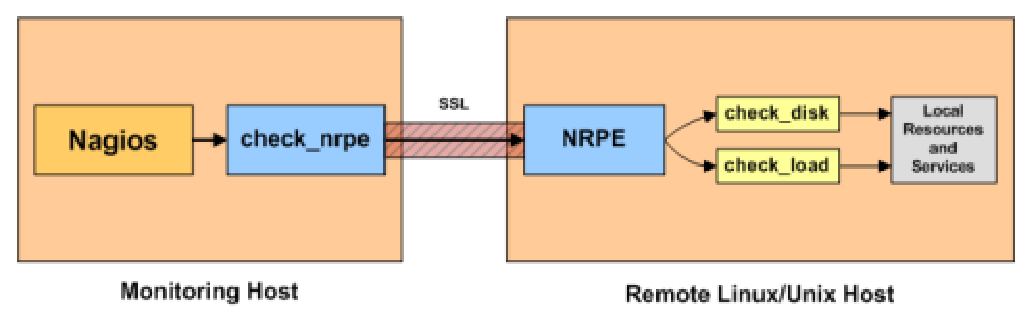
\includegraphics[width=1\linewidth]{pics/nrpe}
	\caption[Funktionsweise NRPE]{Die Funktionsweise von \acrlong{nrpe} (Quelle: \cite{nagioscoreaddons})}
	\label{fig:nrpe}
	\end{figure}

	
	%TODO BI nur mit Addon
	Nagios BPI\footcite{nagiosbpi}
	
	\subsection{Check\_MK - nur ein besser konfigurierbares Nagios?}
	\begin{figure}[!h]
		\centering
		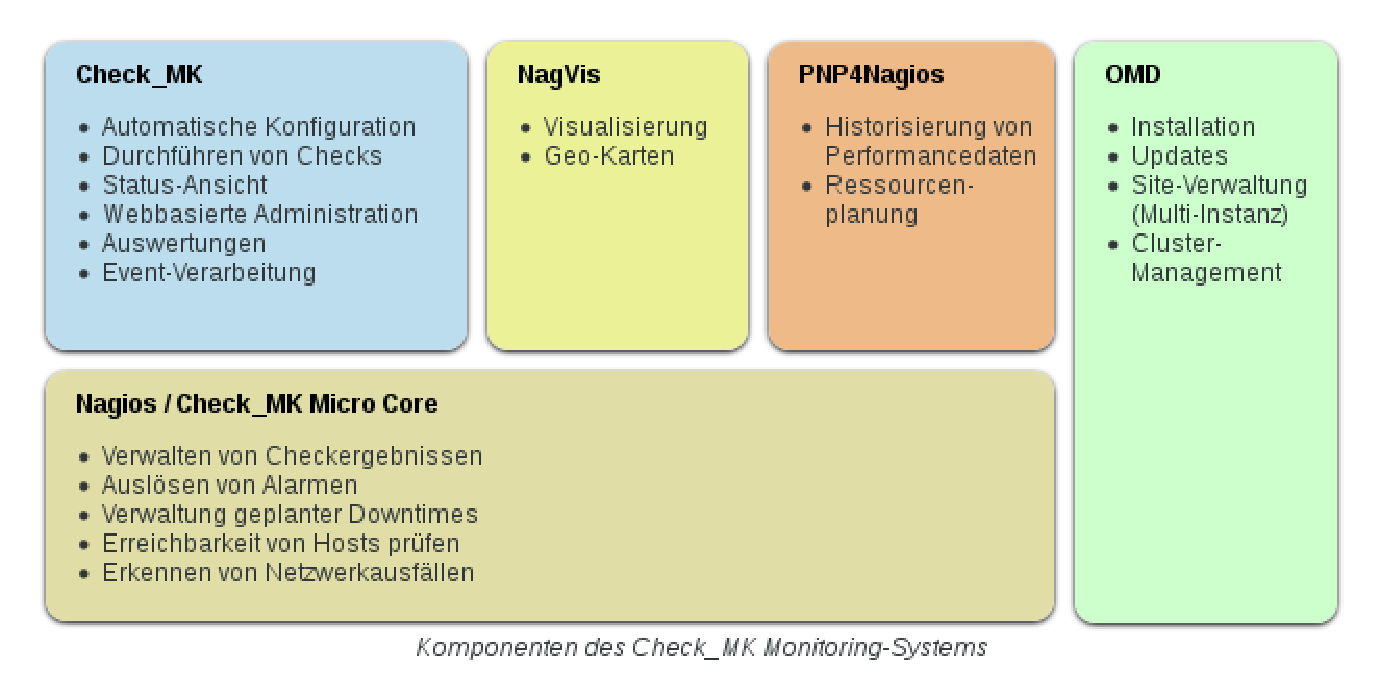
\includegraphics[width=1\textwidth]{pics/checkMKAufbau.eps}
		\caption[Komponenten des Check\_MK Monitoring Systems]{Komponenten des Check\_MK Monitoring Systems (Quelle: \cite{checkmkmonitoringpic})}
		\label{fig:checkmk}
	\end{figure}
	\begin{figure}[!h]
		\centering
		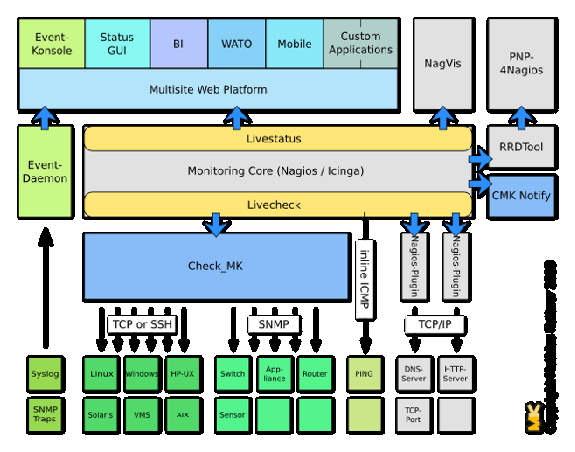
\includegraphics[width=1\textwidth]{pics/OMD_Schema.eps}
		\caption[Aufbau von Check\_MK]{Aufbau von Check\_MK (Quelle: \cite{checkmk})}
		\label{fig:checkmkaufbau}
	\end{figure}
	\clearpage
	
	\section{Logfile Monitoring}
	%TODO Erläuterung welche Tools, es geben würde, warum gerade ELK? Heißester Shit aufm Markt
	\subsection{Syslog-ng und Rsyslog}
	Der erste Gedanke fällt hierbei auf die in den bisherigen BS Vorlesungen gelernten Technologien, weshalb ich hier von dem Schema ein Tool aus der offenen und eines aus der kommerziellen Welt abweichen möchte.
	Problematisch in nicht homogenen Umgebungen mit verschiedenen Versionen aktueller Distributionen, weil systemd...ELK Stack ist hier besser weil vielseitiger
	\footcite{systemd2015}
	%TODO Auch Nagios könnte Logfile Monitoring
	%\subsection{Splunk Monitoring}
	\subsection{Elasticsearch - Logstash - Kibana}
	Oftmals auch \acrshort{elk} oder ELK-Stack genannt sind eigentlich die drei voneinander unabhängige Tools \acrlong{elk}.Um die Funktionsweise und die Integration in unser Monitoring besser erklären zu können, werden die einzelnen Tools mit ihren Möglichkeiten in den folgenden Unterkapiteln kurz vorgestellt und im Anschluß daran ihr Zusammenspiel untereinander und mit dem Monitoring erläutert.
	\subsubsection{Elasticsearch}
	Elasticsearch ist eine auf Apache Lucene basierende Suchmaschine.\footcite{elasticsearch}
	\subsubsection{Logstash}
	Logstash \footcite{logstash}
	%TODO Shipper, Verschlüsselung (Filebeat)
	\subsubsection{Kibana}
	Kibana kann mit dem Elasticsearch \acrshort{rest} \acrshort{api}s umgehen \footcite{kibana}
	\begin{figure}[h!]
		\centering
		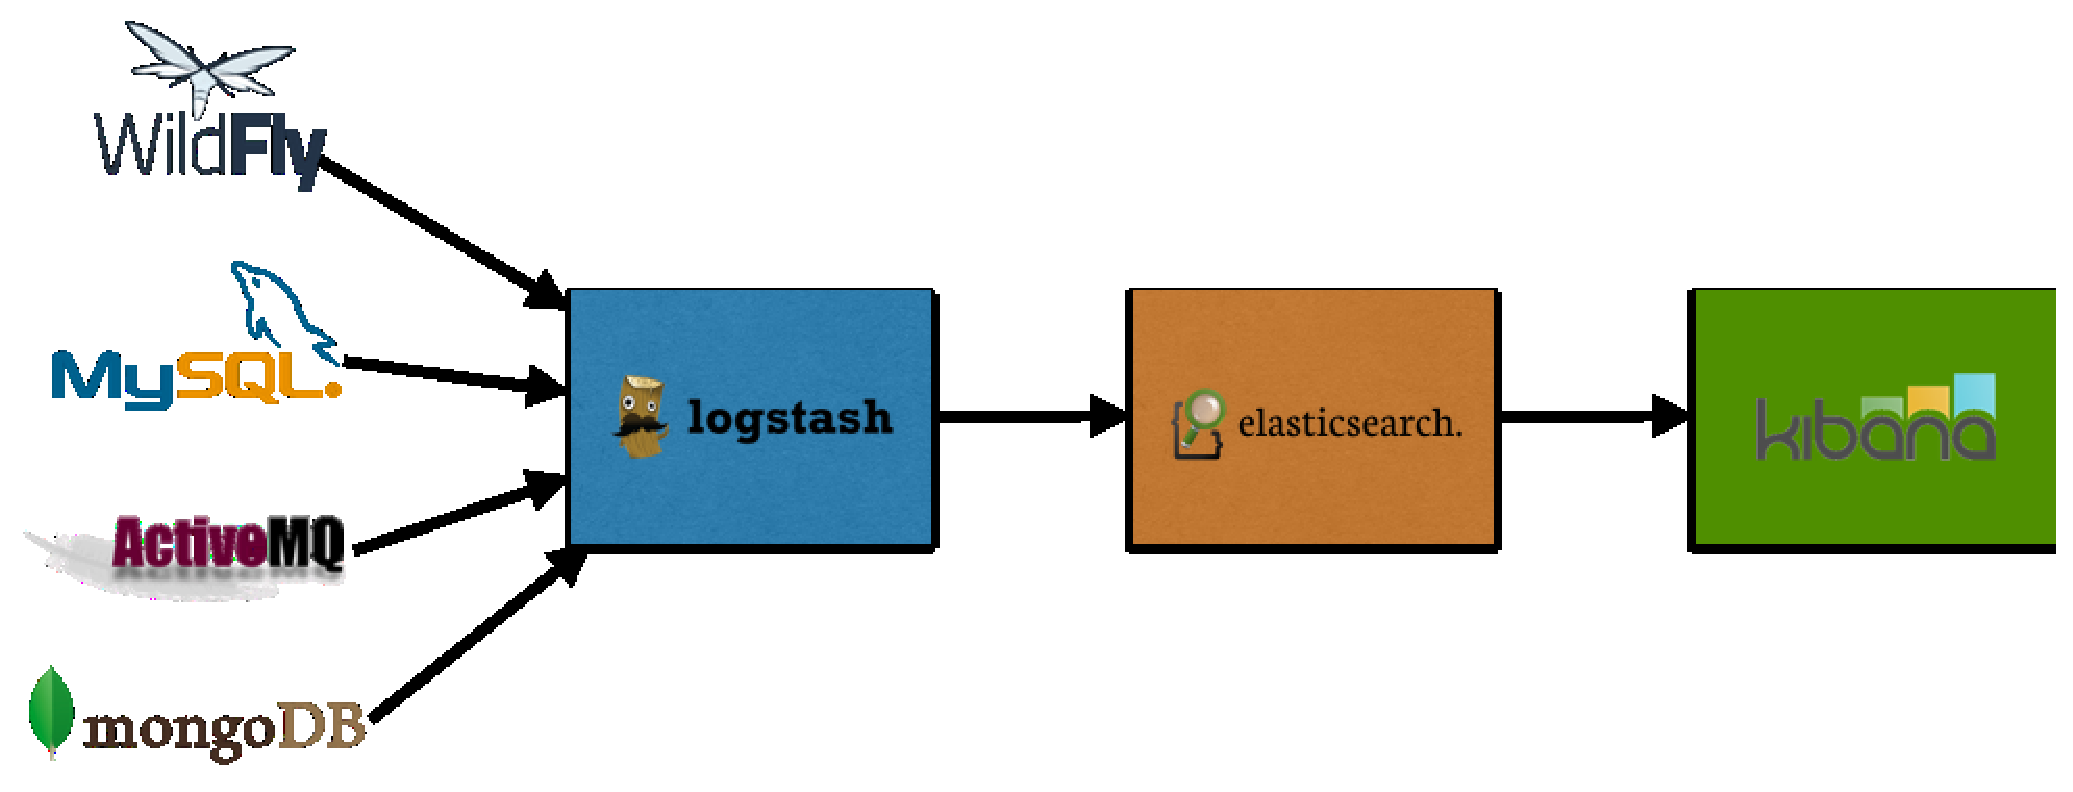
\includegraphics[width=1\textwidth]{pics/elk-stack.eps}
		\caption[Aufbau eines Elasticsearch - Logstash - Kibana Stacks]{Aufbau eines Elasticsearch - Logstash - Kibana Stacks (Quelle: \textcite{elkstackpic})}
		\label{fig:elk}
	\end{figure}
	\clearpage
	%TODO Netways Präsentation für Integration in Nagios
	\chapter{Praktische Vorstellung der Funktionalität eines Monitoring Systems}
	\section{Grundlegende Überlegungen}
	Um kurz noch einen praktischen Einblick in die verwendete Software zu geben wird sich der folgende Teil mit dem praktischen Aufbau einer kleinen \glqq Spielwiese\grqq beschäftigen. 
	
	Es wird auf Basis eines kleinen Versuchsaufbaus, der komplette Prozess (wie in Kapitel 3 beschrieben )bis zu einem fertigen Monitoring durchlaufen.
	\subsection{Versuchsaufbau}
	Im wesentlichen besteht dieser Aufbau aus zwei virtuellen Maschinen die mittels VirtualBox realisiert wurden und einem entfernten Server der bei einem Hoster in einem Rechenzentrum steht. Mit den beiden virtuellen Maschinen werden Server in einem Rechenzentrum simuliert, diese stehen in einem nach außen abgeschotteten Netz, die Datenübertragung bedarf deshalb keiner besonderer Sicherheitsvorkehrungen, der entfernte Server ist nur übers Internet erreichbar (potentiell unsicher!) und die Übertragung der Daten bedarf deshalb einer Verschlüsselung.
	\subsection{Was soll überwacht werden?}
	Wir wollen Performancedaten \& Verfügbarkeit der Systeme überwachen, realisieren als grundlegende und erweiterte Überwachung.
	\subsection{Wie kann überwacht werden?}
	Im wesentlichen werden wir uns bei der Überwachung auf die Daten aus dem Check\_MK Agenten verlassen, dieser betreibt aktive Überwachung.
	Die Log Dateien werden beim Auftreten bestimmter Patterns in die Überwachung übertragen (passive Überwachung). 
	\subsection{Wer soll im Fehlerfall benachrichtigt werden?}
	
	\subsection{Welche \acrlong{sla}s existieren bereits?}
	Für 
	\subsection{Welche Software ist für meine Zwecke am besten geeignet?}
	\section{Grundlegende Beschreibung der verwendeten Systeme}
	\subsection{verwendete Software}
	Als Betriebssystem auf dem Überwachungsrechner kommt Debian 8. zum Einsatz, dies hat den Grund, das Check\_MK in Verbindung mit SuSE beim Aufbau einige Probleme mit fehlenden Paketen hatte, diese Pakete selbst mittels SuSE's \acrfull{obs} zu bauen wäre möglich gewesen.
	%TODO warum nicht passiert?
	 Der entfernte Rechner der per check\_by\_ssh abgefragt wird ist ein virtueller Server bei einem großen Hoster, als Betriebssystem läuft auf diesem Rechner Opensuse 13.2 (64bit) mit der für Webserver üblichen Software (LAMP-Stack = Linux Apache Mysql PHP) und zusätzliche zwei Java Anwendungen (Jenkins \& Sonarqube) mit ihren eigenen Applicationservern. An zusätzlicher überwachter Sicherheitssoftware ist Fail2Ban\footcite{fail2ban} installiert, bei Fail2Ban handelt es sich um eine Sicherheitssoftware, die das Systemlog (\path{/var/log/messages}) auf bestimmte Muster durchsuchen, wenn sich der gleiche User (identifiziert durch die IP) mehrmals hintereinander mit einer bestimmten Fehlermeldung im Syslog auftreten, dann wird die IP über die Firewall gesperrt. \\
	\begin{table}[h] %Quelle: http://www.weinelt.de/latex/table.html
	\begin{center}
	\begin{tabular}{|c|c|c|}
	\hline 
	Eingesetzte Software & Version & Client oder Server \\ 
	\hline 
	VirtualBox & 5.0.14 & Virtualisierungslösung\\
	\hline
	Opensuse & 13.2 & Server\\ 
	\hline 
	Opensuse & Leap 42.1 & Client\\
	\hline
	Apache & 2.4 & Server\\
	\hline
	\acrshort{omd} & 2.11.20160108-labs-edition & Server\\
	\hline
	\end{tabular} 
	\caption[Eingesetzte Softwareversionen]{Für den praktischen Teil der Arbeit eingesetzte Softwareversionen mit ihrem Einsatzort}
	\end{center}
	\end{table}
	\subsection{Installation}
	Um die Software und eventuelle Aktualisierungen permanent verfügbar zu haben, empfiehlt es sich das angebotene Repository \footcite{omdrepo} einzubinden, beim verwendeten OpenSuse funktioniert das wie in Listing 4.1 Zeile 1 gezeigt. Anschließend muss die Software mitsamt ihren Abhängigkeiten installiert werden, dies wird mittels des Paketmanagers \textit{zypper} mit dem wir eben schon das Repository eingehängt haben realisiert (Listing 4.1, Zeile 2). Nach dem Abschluß der Paketinstallationen ist die \acrshort{omd} einsatzbereit.
	\begin{lstlisting}[language=bash, caption=Konfiguration eines Repositories und Installation der \acrfull{omd}]	

	dpkg -i check-mk-raw-1.2.6p15-sles12-34.x86_64.deb
	apt-get -f install
	omd setup
	\end{lstlisting}
	\subsection{Konfiguration}
	
	\section{Performancemonitoring}
	\subsection{Überwachung eines entfernten Servers}
	Installation des Agenten
	Kopieren der zusätzlichen Checks
	
	Schlüsseltausch
	\begin{lstlisting}[language=bash]
	root@linux# ssh -i check_mk.key targethost
	\end{lstlisting} \footcite{checkmkCheckBySSH2015}
	\subsection{Überwachung einer Datenbank}
	\section{Service Level Agreement Monitoring}
	%TODO Beschreibung anhand der Verfügbarkeit einer Webseite
	\subsection{Überwachung der Verfügbarkeit einer Datenbank}
	An dieser Stelle widmen wir uns der Überwachung einer MySQL Datenbank. 
	Wegen der aufkommenden Wichtigkeit von In-Memory Datenbanktechnologien sollte hier auch noch eine In-Memory Datenbank überwacht werden, um die Mächtigkeit des Monitoringwerkzeugs zu zeigen.
	MySQL DB und Derby als Beispiel für die Überwachung einer in Memory Datenbank.
	\subsection{Überwachung der Verfügbarkeit einer Webseite}
	\section{Logfile Monitoring}
	
	% Abkürzungsverzeichnis auf einer neuen Seite ausgeben
	%\printnomenclature
	% Literaturverzeichnis ausgeben und als Eintrag gleichwertig mit einem Kapitel ins Inhaltsverzeichnis eintragen
	%\begingroup
	%\nocite{*} %Alle Einträge des Literaturverzeichnisses auch ohne Zitierung ausgeben
	%\addcontentsline{toc}{chapter}{Literatur}
	\printbibliography 
	%\addchaptertocentry{}{Literatur}
	%\addcontentsline{toc}{chapter}{Literatur}
	%\endgroup
	\printglossary[title=Abkürzungsverzeichnis, type=\acronymtype] % prints just the list of acronyms	
	%\printglossary[title=Glossar]
	%\printglossaries	
	\listoffigures % Abbildungsverzeichnis
	%\addchaptertocentry{}{Abbildungsverzeichnis}
	%\listoftables % Verzeichnis der Tabellen
	%\addchaptertocentry{}{Tabellenverzeichnis}
\end{document}